\section{CubeSat Chassis Design}
% % for code listings
% \begin{lstlisting}[style=cstyle, caption=System Architecture Code Example, label=lst:SystemArchitecture8]
% # Your code here
% \end{lstlisting}

% % for figures
% \begin{figure}[htbp] %h-ere t-op b-ottom p-page (separte) -good to allow all htbp to give the compiler more options
%     \centering
%     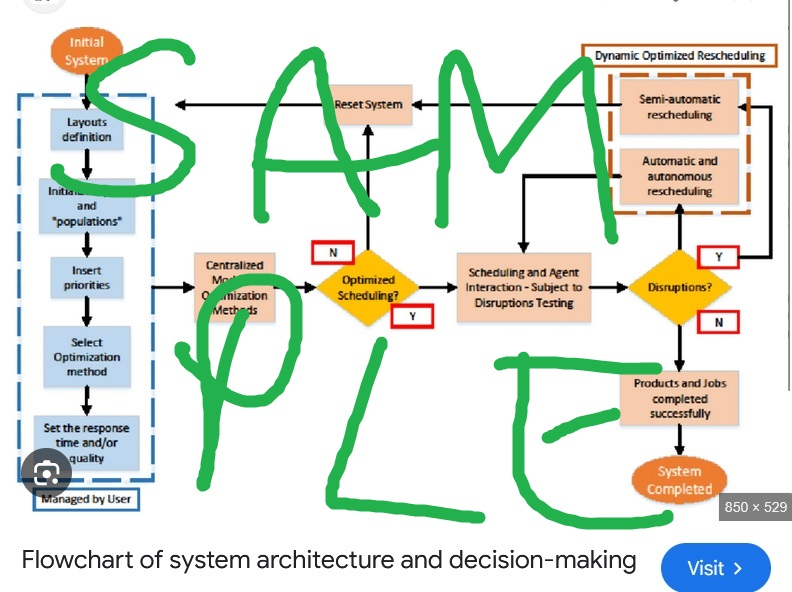
\includegraphics[width=0.6\textwidth]{figures/methodology/system_architecture.jpg}
%     \caption{System Architecture Diagram}
%     \label{fig:system-architecture3}
% \end{figure}

% % Include a flowchart in TEX mode
% \begin{figure}[H]
%     \centering
%     \scalebox{0.8}{ % Scale to 80% of original size
%         % try generating flowcharts as svg in Claude 
% and edit with inkscape instead of this.
% but claude did generate this one so might 
% be useful too but you can't easily make
% small repairs in inkscape


% CNN Transfer Learning Flowchart - Compact Multi-Column Layout
% \begin{figure}[htbp]

\centering
\resizebox{\textwidth}{!}{ % Scale to fit width while maintaining aspect ratio
\begin{tikzpicture}[node distance=0.8cm and 1.5cm, auto]
    % Define a smaller block style
    \tikzset{
      block/.style = {rectangle, draw, fill=blue!20, 
                      text width=7em, text centered, rounded corners, minimum height=1.8em, font=\small},
    }
    
    % Brazilian model training - Column 1
    \node [block] (brazildata) {Download Brazilian coins dataset};
    \node [block, below=of brazildata] (extract) {Extract dataset};
    \node [block, below=of extract] (setup) {Setup directories};
    \node [block, below=of setup] (define) {Define train/val dirs};
    \node [block, below=of define] (create) {Create CNN architecture};
    \node [block, below=of create] (compile) {Compile the CNN};
    \node [block, below=of compile] (train) {Train model};
    \node [block, below=of train] (trained) {Model trained (5 classes)};
    
    % Transfer learning - Column 2 (Middle)
    \node [block, right=2.5cm of brazildata] (freeze) {Freeze all layers};
    \node [block, below=of freeze] (replace) {Replace final layers};
    \node [block, below=of replace] (add) {Add regularization and dropout};
    \node [block, below=of add] (output) {New output layer (8 classes)};
    \node [block, below=of output] (finaltrain) {Train and fine-tune};
    \node [block, below=of finaltrain] (inference) {Perform inference on new coins};
    
    % UK data preparation - Column 3 (Right)
    \node [block, right=2.5cm of freeze] (ukdata) {Download UK coins dataset};
    \node [block, below=of ukdata] (ukextract) {Extract UK dataset};
    \node [block, below=of ukextract] (uksetup) {Setup UK directories};
    \node [block, below=of uksetup] (ukgen) {Create data generators (80/20 split)};
    
    % Connect all nodes with arrows
    \path [line] (brazildata) -- (extract);
    \path [line] (extract) -- (setup);
    \path [line] (setup) -- (define);
    \path [line] (define) -- (create);
    \path [line] (create) -- (compile);
    \path [line] (compile) -- (train);
    \path [line] (train) -- (trained);
    
    \path [line] (ukdata) -- (ukextract);
    \path [line] (ukextract) -- (uksetup);
    \path [line] (uksetup) -- (ukgen);
    
    % Connect the columns
    \path [line] (trained) -- node[midway, above] {Transfer} (freeze);
    \path [line] (ukgen) |- (finaltrain);
    
    % Connect middle column
    \path [line] (freeze) -- (replace);
    \path [line] (replace) -- (add);
    \path [line] (add) -- (output);
    \path [line] (output) -- (finaltrain);
    \path [line] (finaltrain) -- (inference);
    
    % Group boxes to show different stages with smaller padding
    \begin{pgfonlayer}{background}
        \node[group={[yshift=0.3cm]above:Brazilian Model Training}, fit={(brazildata) (extract) (setup) (define) (create) (compile) (train) (trained)}, inner sep=0.2cm] {};
        \node[group={[yshift=0.3cm]above:UK Data Preparation}, fit={(ukdata) (ukextract) (uksetup) (ukgen)}, inner sep=0.2cm] {};
        \node[group={[yshift=0.3cm]above:Transfer Learning}, fit={(freeze) (replace) (add) (output) (finaltrain) (inference)}, inner sep=0.2cm] {};
    \end{pgfonlayer}
\end{tikzpicture}
}
% \caption{CNN Transfer Learning Flowchart: Brazilian to UK Coins}
% \label{fig:cnn-flowchart}
% \end{figure} % \input is for tex files \includegraphics is for images
%     }
%     \caption{System Design Overview Flowchart}
%     \label{fig:decriptiveLabel22} % descriptive to call in text with \ref{fig:decriptiveLabel22}
% \end{figure}
For the purposes of visualization, there were 2 potential designs for the CubeSat chassis. The CubeSat chassis were design dependant on where the PCB would be mounted. The first CubeSat chassis design was taken from GrabCAD.com and an aperture is mounted to this design to show where they would be mounted. The second CubeSat chassis was based on a design found online and recreated as much as possible, however this did not have any measurements given so dimensions were assumed.

\subsection{CubeSat Chassis Design 1}

\begin{figure}[htbp]
    \centering
    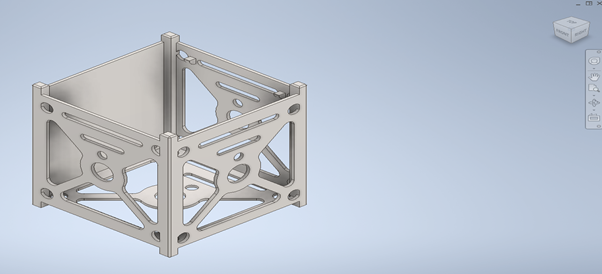
\includegraphics[width=\textwidth]{chapters/methodology/CubeSatDesign/Fig1CAD.png}
    \caption{Front view of the first CubeSat chassis design}
    \label{fig:cubesat-chassis1-front}
    \end{figure}

    \begin{figure}[htbp]
    \centering
    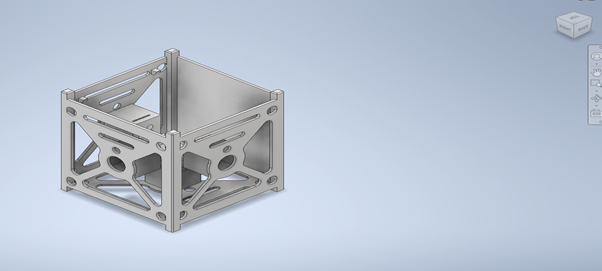
\includegraphics[width=\textwidth]{chapters/methodology/CubeSatDesign/Fig2CAD.png}
    \caption{Angular view of the first CubeSat chassis design}
    \label{fig:cubesat-chassis1-angle}
    \end{figure}

    The first design taken from \url{https://grabcad.com/library/cubesat-1u-5} as seen in Figure~\ref{fig:cubesat-chassis1-front} has exposed holes made to allow for easy removal, the circular holes at the centre are to let the light to expose to the aperture where the PCB photodiodes are located. The software used to show these are AutoCAD Inventor, with a different angle and the aperture shown in Figure~\ref{fig:cubesat-chassis1-angle}.


\subsection{CubeSat Chassis Design 2}
The second hypothetical design is a much more basic skeleton frame made to house the aperture as seen below in Figure~\ref{fig:cubesat-chassis2-front} and Figure~\ref{fig:cubesat-chassis2-angle}.

\begin{figure}[htbp]
\centering
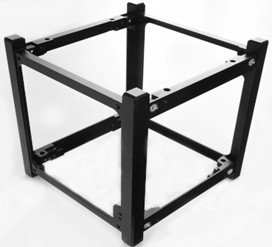
\includegraphics[width=0.7\textwidth]{chapters/methodology/CubeSatDesign/Fig3Real.jpg}
\caption{Front view of 1U Cubesat Skeleton Chassis}
\label{fig:cubesat-chassis2-front}
\end{figure}

\begin{figure}[htbp]
\centering
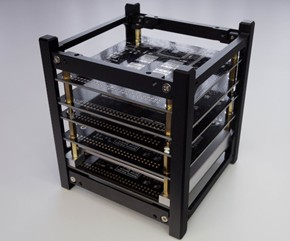
\includegraphics[width=0.7\textwidth]{chapters/methodology/CubeSatDesign/Fig4Real.jpg}
\caption{Angular view of 1U Cubesat Skeleton Chassis}
\label{fig:cubesat-chassis2-angle}
\end{figure}

This was recreated in inventor with rough estimation on the thickness of the PCBs and skeletons itself and the apertures. The PCBs are mounted on top of each other compared to being the aperture housing the PCB mounted on each side of the CubeSat, the PCB cannot be more than 96$\times$96 mm. As seen below in Figure~\ref{fig:cubesat-chassis2-without-pcb} and Figure~\ref{fig:cubesat-chassis2-with-aperture}, are the CubeSat Chassis with and without the PCBs, additional angles and drawings are found in the appendix.
\begin{figure}[htbp]
\centering
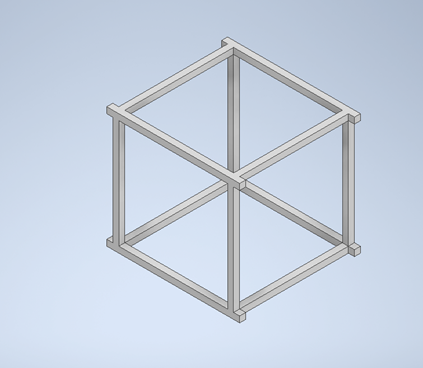
\includegraphics[width=0.8\textwidth]{chapters/methodology/CubeSatDesign/Fig5CAD.png}
\caption{Second chassis design without PCBs}
\label{fig:cubesat-chassis2-without-pcb}
\end{figure}

\begin{figure}[htbp]
\centering
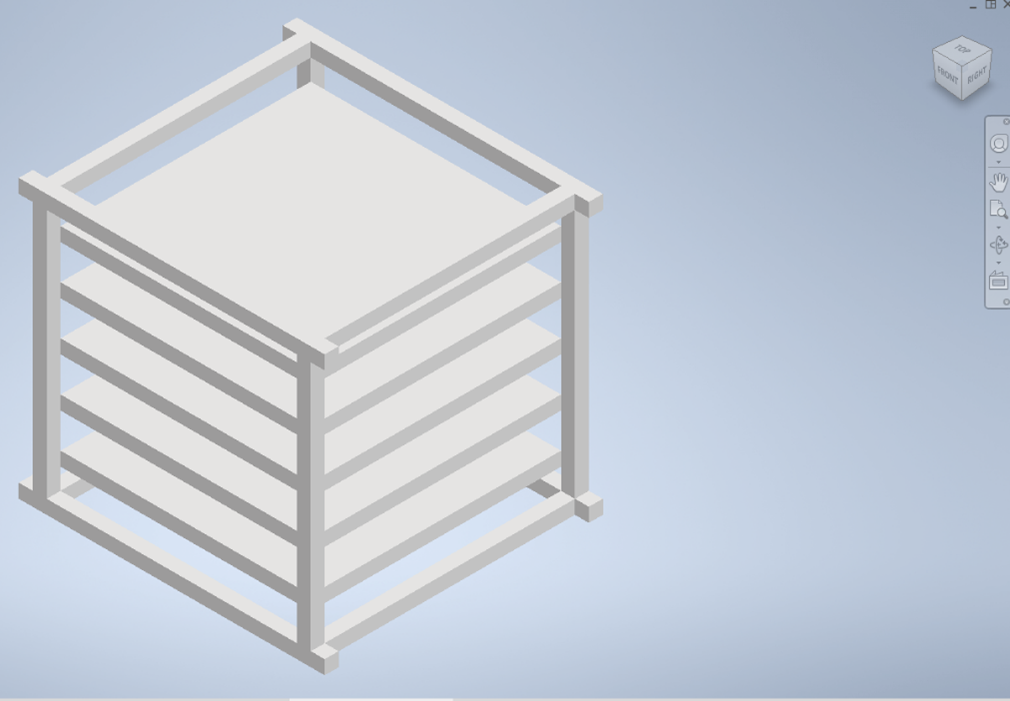
\includegraphics[width=0.8\textwidth]{chapters/methodology/CubeSatDesign/Fig6CAD.png}
\caption{Chassis with the aperture}
\label{fig:cubesat-chassis2-with-aperture}
\end{figure}